\chapter{Introduction}
\label{cha:introduction}
This chapter provides the necessary background material and details the organization of my proposed work.

\section{Multi-modality}
\subsection{Modalities - Definition and Introduction}
\textit{Modality refers to the way something happens around us or is perceived by humans} \cite{Baltruaitis2017MultimodalML}. The world around us is composed of multiple sensory modalities, as listed below, with enabled capabilities:
\begin{itemize}
    \item \textbf{Visual:} Watching objects and events in the current visual scene
    \item \textbf{Language:} Verbal interactions with other humans 
    \item \textbf{Audio:} Speaking and hearing environmental sounds 
    \item \textbf{Touch:} Feeling texture of objects 
    \item \textbf{Smell:} Distinguishing between pleasant and unpleasant odors.
\end{itemize}
In artificial intelligence, a given task is considered multi-modal if multiple sensory modalities are needed to solve the same. The goal of artificial intelligence is to develop autonomous agents capable of processing information from a wide variety of input modalities for tackling complex reasoning tasks. As mentioned by Liang et al. \cite{Liang2022FoundationsAR}, the key properties associated with learning from multimodal data are listed as follows:
\begin{itemize}
    \item \textbf{Heterogeneity:} Heterogeneous nature of different modalities due to diversity in qualities, structures, and representations
    \item \textbf{Connectedness:} Shared/common information between different modalities due to inter-related nature.
    \item \textbf{Interaction:} Existence of optimal interactions/fusions between different modalities, suitable for particular task.
\end{itemize}
Based on the above properties associated with multiple modalities, the major challenges in multimodal learning \cite{Liang2022FoundationsAR} can be summarized below:

\begin{itemize}
    \item \textbf{Representation:} Learning representations through fusion mechanisms that capture the heterogeneity of the modalities along with the shared information. For example, language is considered symbolic due to its word-based composition, whereas audio and visual modalities are represented through signals.
    \item \textbf{Alignment:} Identifying relationships between (sub) elements of different modalities. This requires similarity computation between different modalities along with the handling of long-term dependencies.
    \item \textbf{Reasoning:} Combining knowledge from multiple sources (including external, i.e. knowledge graphs) in a multi-step inference process by exploiting the task structure.
    \item \textbf{Generation:} Translating between different modalities and summarization of multimodal data by preserving the salient content.
    \item \textbf{Transference:} Transferring cross-modal knowledge from secondary modalities to the primary modality in the presence of noise or limited data.
\end{itemize}

In this work, we deal with the alignment, reasoning, and transference challenges associated with multi-modal learning.
    
\subsection{Rise of multi-modal content}
Give a sense of media data that is inherently multi-modal and rising in content

\section{What is context ?}
In computer vision, context \cite{contextvision} refers to any relevant information encompassing the attributes of the object and event considered, along with other entities (objects and events) in the given scene, both visual and non-visual. Contextual information enables a wide variety of tasks, including object recognition, human affect perception, and salient event detection in videos, by providing additional cues needed for accurate inference. For example, the visual scene in a given image provides the necessary contextual information to detect commonly co-occurring objects along with any atypical placements. In terms of object placements, utensils are more likely to be found in the kitchen as compared to bedrooms or stadiums. An example of context providing the required information to improve object recognition under challenging conditions (poor lighting, image blurring, ) is shown in Fig \ref{object recognition}. The blurred object (marked by a red circle), when viewed in isolation, is not recognizable. However, when the object is placed in the context of the entire visual scene i.e. office, we can see that it is likely to be a keyboard.
\begin{figure}
    \centering 
     
\includegraphics[width=0.6\linewidth]{figures/blurred_object.png}
     \caption{ \textbf{LEFT:} A blurred object (marked in red circle), when viewed in isolation, is not recognizable. \textbf{RIGHT:} Contextual information in the form of the visual scene helps in recognition. }
     \label{object recognition}
\end{figure}

The broad organization of different context sources, along with associated levels is shown in Fig \ref{Context_type}.
\begin{figure}[t]
  \centering
  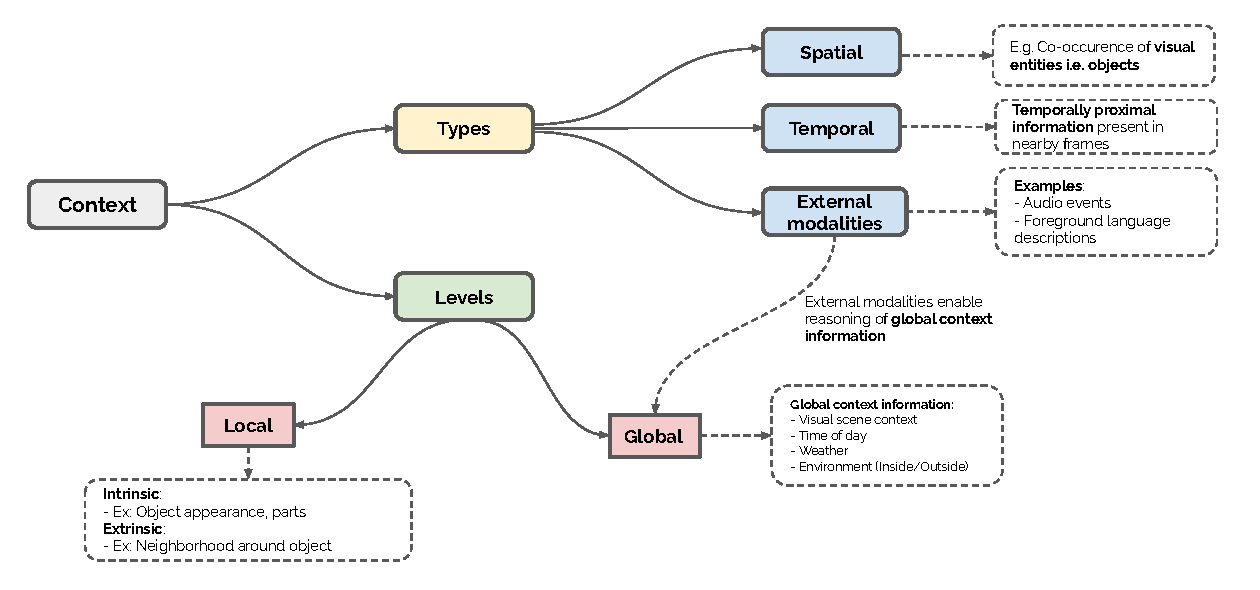
\includegraphics[width=\linewidth]{figures/Context_type.pdf}
  \caption{Variations in types and levels of context. Outline of context levels and types inspired from Fig 5 in \cite{contextvision}.}
  \label{Context_type}
\end{figure}
Context can be broadly divided into three types as follows:

\subsection{Spatial context}
Spatial context refers can be defined as the \textit{possibility of finding objects located at certain positions in the scene w.r.t other proximal objects}. For example, a ship can be found floating at sea rather than on a highway.
Spatial context can be further subdivided into the following major classes:
\begin{itemize}
    \item  \textbf{Spatial co-occurrence}: Spatial co-occurrence can be leveraged through co-occurrences of object labels in the same visual scene. Rabinovich et.al \cite{Rabinovich2007ObjectsIC} utilized co-occurrence statistics between labels in a CRF-based framework to refine object detections in a given visual scene. Further, Wang et al. \cite{Wang2007ShapeAA} expanded the idea of co-occurrence by providing a probability distribution of labels over different regions based on a given pixel location. Yang et.al \cite{Faceness-Net} explored fine-grained relative spatial information between facial parts i.e., placement of nose, mouth for face detection. 
    \item  \textbf{Direction and toplogical relations}: 2-D spatial relations between entities can be described through direction and topological-based relations \cite{Marques2010ContextMI}. Directional relations deal with the proximity of one object with other objects in terms of other entities based on relative terms like \textit{"near"}, \textit{"above"}, \textit{"below"}. Whereas topological relations are concerned with the neighborhood of the objects in terms of overlap/containment with distinct regions i.e. exterior, boundary and interior.
    \item  \textbf{Semantic driven spatial context}: Semantic context restricts the space of possible spatial contextual relations in a given scene to a set of valid ones. The usage of semantic context between proximal objects enables correction of mislabeling in images \cite{Rabinovich2007ObjectsIC}, and accurate discovery of all possible valid relations between objects through scene graphs \cite{Chang2021ACS}. An example of a scene graph with entities and semantic relations obtained after message-passing operations \cite{Xu2017SceneGG} is shown in Fig \ref{scenegraph}.
    \begin{figure}[h!]
    \centering
        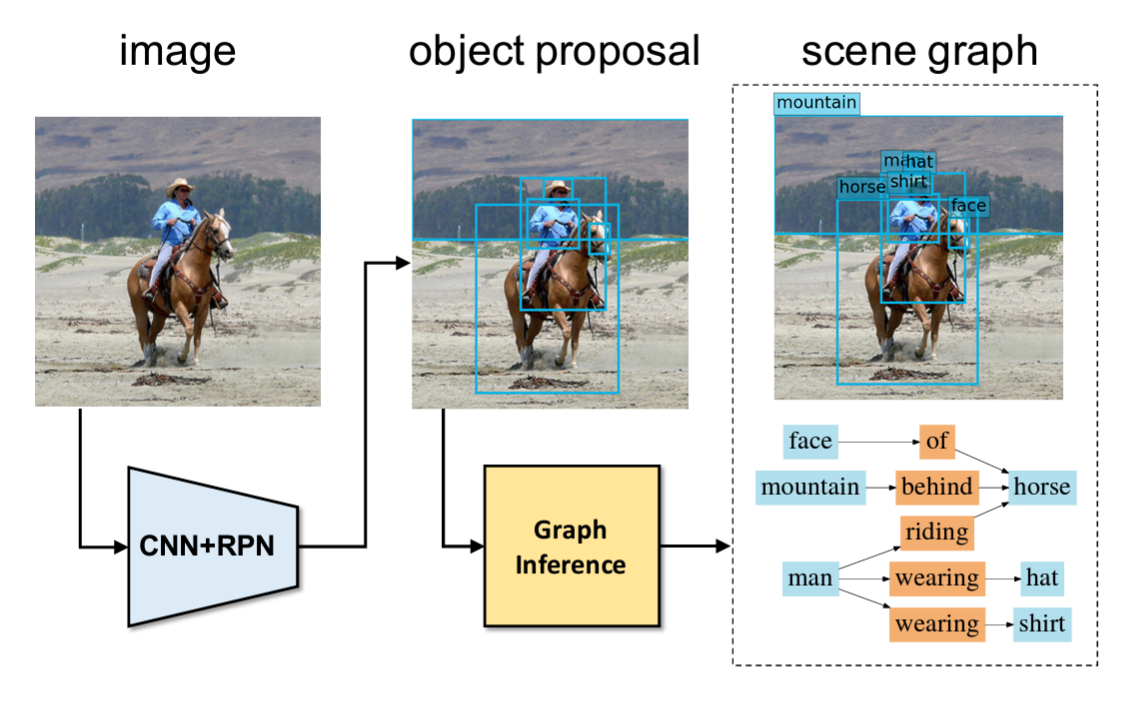
\includegraphics[width=0.5\linewidth]{figures/Scene_graph_outline.png}
        \caption{Sample scene graph obtained after iterative message passing (graph interface) over the region proposals (objects) }
        \label{scenegraph}
    \end{figure}
\end{itemize}

\subsection{Temporal context}
Temporal context refers to the \textit{information present in dynamic content, i.e. nearby or distant frames in videos}. The major subdivisions of temporal context are listed as follows:
\begin{itemize}
\item \textbf{Short-term temporal context:} Short-term temporal context relies on information present in nearby frames, which can be a short temporal window centered on the current frame or previous frame. The temporal context within a short window, (usually a few seconds) enables general video understanding tasks, including action recognition \cite{Carreira2017QuoVA}, pedestrian tracking \cite{Yan2019LearningCG}, human-object interaction \cite{Ji2021DetectingHR}. 
\item \textbf{Long-term temporal context:} Instead of limiting to nearby frames, long-term temporal context deals with temporal scale spanning from hours to months/years. General media-focused tasks based on movies \cite{Wu2021TowardsLV,Soldan2021MADAS} rely on long-form narratives (usually minutes to hours) for understanding character interactions, event dynamics, and broad semantics, including genre, etc. For tasks like species monitoring, temporal information over extended periods of time (months or years) is required for accurate identification \cite{Beery2019ContextRL}. 
\end{itemize}
In spite of clear divisions between short-term and long-term temporal contexts based on the duration of information, certain narrative-driven videos in media, i.e., advertisements, contain: 
\begin{itemize}
\item Rapid changes in short-term contextual information based on shots. 
\item Long-term contextual association between the shots based on an integrated narrative.
\end{itemize}
\subsection{External modalities}
Apart from visual-only information, modalities such as audio, language, and prior weather information also provide relevant contextual information for various reasoning tasks. For example, in the case of audio-visual tasks, the audio associated with an entity, i.e., dog barking, can help us estimate the proximity of the sound source and localize it in the given video \cite{Tian2018AudioVisualEL}. Further usage of audio modality as an additional contextual source for visual tasks has been explored in floorplan design \cite{purushwalkam2020audio} and audio-visual navigation for virtual agents \cite{chen2020soundspaces}. For various vision-language tasks like temporal grounding, natural language queries can be used as contextual inputs to isolate regions of interest in unconstrained videos \cite{Zhang2022TemporalSG}. Besides language and audio, additional contextual information available through thermal sensors \cite{Seymour2017AutomatedDA} is used to augment the visually captured data for improving wildlife detection in remote areas.

\subsection{Local context}

\subsection{Global context}

\section{Context-driven multi-modal understanding}
\section{Organization of proposal}

